\chapter*{Filtrace obrazových signálů} \label{sec:filtrace}

Filtrace je jednou ze základních metod úpravy signálů (včetně signálů reprezentujících obrazy) spočívající v úpravě kmitočtového spektra. V principu lze filtraci provádět dvěma postupy: nerekurzivně a rekurzivně. Uvažujme prostor diskrétních signálů. Nerekurzivní filtry vytvářejí výstupní signál v každém bodě jako lineární kombinaci vzorků signálu vstupního. Impulzová charakteristika nerekurzivních filtrů obsahuje vždy jen konečný počet nenulových hodnot, protože jinak by je nebylo možné prakticky realizovat. Nerekurzivní filtry jsou proto také označovány jako filtry FIR (finite-extent impulse response). Rekurzivní filtry naproti tomu předepisují vztah mezi vstupním a výstupním signálem obecněji: výstupní signál v každém bodě je lineární kombinací vzorků nejen signálu vstupního, ale také právě určovaného signálu výstupního. Jako rekurzivní lze realizovat také filtry, jejichž impulzová charakteristika obsahuje nekonečný počet nenulových hodnot. Rekurzivní filtry proto také bývají označovány jako filtry IIR (infinite-extent impulse response). Problematice nerekurzivní i rekurzivní filtrace je věnována tato kapitola. Kromě teoretických základů uvedeme také některé praktické metody návrhu filtrů, včetně metod využívajících stochastického přístupu.

\section*{Nerekurzivní filtrace}

Nechť \textit{f}(\textit{m},\textit{n}) je diskrétní vstupní signál a \textit{h}(\textit{m},\textit{n}) nechť je impulzová charakteristika filtru. Nerekurzivní filtrací rozumíme úpravu signálu podle předpisu

\begin{equation} \label{eq:5_1}
    g(m, n) = f(m, n) * h(m, n).
\end{equation}

Provedeme-li Fourierovu transformaci rovnice \eqref{eq:5_1}, získáváme vztah

\begin{equation} \label{eq:5_2}
    G(k, l) = F(k, l) * H(k, l).
\end{equation}

Z~rovnice \eqref{eq:5_2} je patrné, že filtrace provádí úpravu frekvenčního spektra signálu. Tato představa bývá ostatně dosti často primární. Často požadujeme, aby filtr modifikoval frekvenční spektrum signálu jistým předepsaným způsobem, tj. aby měl jistou požadovanou frekvenční charakteristiku.

\subsection*{Realizace nerekurzivního filtru v~prostorové a frekvenční doméně}

V praxi se výpočet filtrace provádí jak v doméně prostorové podle vztahu \eqref{eq:5_1}, tak v doméně frekvenční podle vztahu \eqref{eq:5_2}. Jedním z faktorů, které ovlivňují volbu postupu, je časová složitost výpočtu. Uvedeme příklad časové rozvahy. Předpokládejme, že máme provést filtraci dle vztahu \eqref{eq:5_1} a že funkce \textit{f}, \textit{h} jsou nenulové nad čtvercovými oblastmi o rozměrech \textit{M}$\times$\textit{M} a \textit{R}$\times$\textit{R} bodů. Předpokládejme, že vstupní signál \textit{f} i impulzová charakteristika \textit{h} filtru jsou reálné, což bývá v~praxi často splněno. Časovou složitost měříme počtem reálných násobení. Protože při praktické realizaci konvoluce máme vypočítat \textit{M}$^2$ hodnot a protože výpočet každé z~nich vyžaduje \textit{R}$^2$ násobení, dostáváme pro časovou složitost \textit{C}$_\mathrm{S}$ filtrace realizované v prostorové doméně vztah

\begin{equation} \label{eq:5_3}
    C_\mathrm{S} = M^2 R^2.
\end{equation}

Při provádění filtrace ve frekvenční doméně je třeba provést Fourierovu transformaci vstupního signálu, pak součin na pravé straně vztahu \eqref{eq:5_2} a konečně zpětnou Fourierovu transformaci. Předpokládáme, že frekvenční charakteristiku \textit{H}(\textit{k},\textit{l}) použitého filtru známe předem a že ji není nutné počítat. Protože přechod od vztahu \eqref{eq:5_1} ke vztahu \eqref{eq:5_2} předpokládá použití cyklické konvoluce, převedeme výpočet konvoluce lineární (v praktických aplikacích se konvoluce ve vztahu (5.1) dosti často uvažuje lineární) na výpočet konvoluce cyklické tak, jak jsme již dříve popsali v~odstavci \ref{sec:diskretni_konvoluce}. Zaveďme označení \textit{Q}=\textit{M}+\textit{R}$-$1. Z odstavce (TOTO V NOVYCH SCRIPTECH CHYBI) XXX 2.3.5 víme, že časová složitost rychlé Fourierovy transformace je 3\textit{Q}$^2$log$_2$\textit{Q}/4 komplexních násobení - tj. 3\textit{Q}$^2$log$_2$\textit{Q} násobení reálných (jedno násobení komplexní vyžaduje čtyři násobení reálná). Celková časová složitost \textit{C}$_\mathrm{F}$ filtrace realizované ve frekvenční doméně měřená počtem reálných násobení tedy je

\begin{equation} \label{eq:5_4}
    C_\mathrm{F} = Q^2 ( 3 \log_2 Q + 4 + 3 \log_2 Q ) = Q^2 ( 4 + 6 \log_2 Q ).
\end{equation}

Porovnáním vztahů \eqref{eq:5_3} a \eqref{eq:5_4} zjišťujeme, že provedení filtrace ve frekvenční doméně je výhodnější, jestliže platí

\begin{equation} \label{eq:5_5}
    R > \sqrt{4 + 6 \log_2 Q}.
\end{equation}

Např. pro \textit{Q}=1024 vychází, že filtrace ve frekvenční doméně je při uvedených kriteriích výhodnější pro \textit{R}$>$8.

\subsection*{Filtry s nulovou fází}

Úpravu frekvenčního spektra intuitivně chápeme tak, že se filtrací mění amplituda jednotlivých frekvenčních složek signálu, nikoli však jejich fáze. Předpokládáme tedy, že frekvenční charakteristika filtru je reálná (obecněji můžeme na takový filtr pohlížet jako na filtr, jehož frekvenční charakteristika má nulové imaginární složky, a proto jej nazýváme filtrem s nulovou fází). Oprávněnost uvedeného požadavku je stvrzována praktickými zkušenostmi - při zpracování obrazu filtry, jejichž frekvenční charakteristika má nenulové imaginární složky, lze subjektivně zaznamenat nežádoucí degradace obrazu. Podmínku nulové fáze filtru ve frekvenční doméně můžeme zapsat pomocí vztahu

\begin{equation} \label{eq:5_6}
    H(k, l) = H^*(k, l).
\end{equation}

S využitím předpisu \eqref{eq:2_39} pro Fourierovou transformaci odtud snadno získáváme podmínku

\begin{equation} \label{eq:5_7}
    h(m, n) = h^*(-m, -n).
\end{equation}

Vidíme tedy, že podmínka nulové fáze frekvenční charakteristiky filtru vyžaduje, aby impulzová charakteristika filtru byla centrovaná kolem počátku podle vztahu \eqref{eq:5_7}. Při filtraci obrazů je někdy možné volit impulzovou charakteristiku filtru na základě intuice. I v~takovém případě lze ovšem z výše popsaných důvodů doporučit respektování vztahu \eqref{eq:5_7}. 

\subsection*{Návrh filtru s využitím výřezové funkce}

Často chceme v prostorové doméně realizovat filtr, jehož požadovanou impulzovou charakteristiku (označme ji např. \textit{i}(\textit{m},\textit{n})) sice známe, avšak její praktické použití je nevýhodné, protože je nenulová nad příliš rozsáhlou oblastí, což by vedlo k vysoké časové složitosti výpočtu. V těchto případech lze vytvořit aproximaci \textit{h}(\textit{m},\textit{n}) ideální impulzové charakteristiky \textit{i}(\textit{m},\textit{n}) jejím zkrácením pomocí výřezové (okenní) funkce \textit{w}(\textit{m},\textit{n}) podle předpisu

\begin{equation} \label{eq:5_8}
    h(m, n) = i(m, n) w(m, n).
\end{equation}

Návrh filtru nyní spočívá ve volbě vhodného typu výřezové funkce \textit{w} a ve volbě velikosti výřezu tak, aby se vlastnosti filtru dostatečně shodovaly s vlastnostmi požadovaného filtru ideálního. Při volbě výřezové funkce se zpravidla požaduje splnění následujících vlastností:

\begin{equation} \label{eq:5_9}
    w(m, n) = w^*(-m, -n),
\end{equation}

\begin{equation} \label{eq:5_10}
    w(m, n) = w_1(m) w_2(n).
\end{equation}

Místo separability dle vztahu \eqref{eq:5_10} může být někdy požadována funkce rotačně symetrická, což je zajištěno předpisem

\begin{equation} \label{eq:5_11}
    w(m, n) = w_0\left( \sqrt{m^2 + n^2} \right).
\end{equation}

Splnění uvedených vlastností většinou usnadňuje realizaci následného výpočtu. Splnění vlastnosti \eqref{eq:5_9} je předpokladem pro vytvoření filtru s nulovou fází. Separabilita funkce podle \eqref{eq:5_10} ulehčuje např. výpočet Fourierovy transformace. Je totiž

\begin{equation} \label{eq:5_12}
    \mathscr{F} \left\{ w(m, n) \right\} = \mathscr{F} \left\{ w_1(m)w_2(n) \right\} = \mathscr{F} \left\{ w_1(m) \right\} \mathscr{F} \left\{w_2(n) \right\} = W_1(k) W_2(l).
\end{equation}

V praxi se používá mnoha typů výřezových funkcí. Zde uvedeme pouze některé z~nich (dále uvedené funkce mohou být použity na místě funkcí \textit{w}$_1$, \textit{w}$_2$, \textit{w}$_0$, \textit{Q} označuje velikost výřezu):

\noindent obdélník:

\begin{equation} \label{eq:5_13}
    w(n) = \left\{
    \begin{array}{cc}
    1, & |n|<Q \\
    0, & \mathrm{jinak}
    \end{array}
    \right. ,
\end{equation}

\noindent Barlettova funkce:

\begin{equation} \label{eq:5_14}
    w(n) = \left\{
    \begin{array}{cc}
    \left( 1 - \frac{\left| n \right|}{Q} \right) , & |n|<Q \\
    0, & \mathrm{jinak}
    \end{array}
    \right. ,
\end{equation}

\noindent Hanningova funkce:

\begin{equation} \label{eq:5_15}
    w(n) = \left\{
    \begin{array}{cc}
    \frac{1}{2} \left[ 1 + \cos \left( \pi \frac{n}{Q} \right) \right] , & |n|<Q \\
    0, & \mathrm{jinak}
    \end{array}
    \right. .
\end{equation}

\begin{figure}[th]
    \begin{center}
        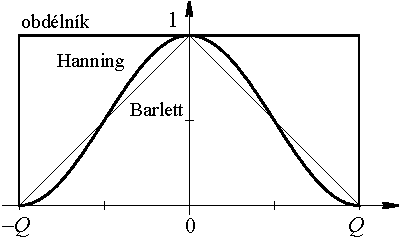
\includegraphics[scale=1.0]{05_filtrace/images/img_5_1.pdf}
    \end{center}
    \caption{Průběh některých výřezových funkcí.}
    \label{img:5_1}
\end{figure}

Průběhy uvedených funkcí jsou znázorněny na obr. \ref{img:5_1}. Průběh frekvenční charakteristiky $\mathscr{F}$\{\textit{i}(\textit{m},\textit{n})\textit{w}(\textit{m},\textit{n})\} lze použít pro posouzení kvality filtru. Uplatníme-li na obě strany rovnice \eqref{eq:5_8} Fourierovu transformaci, pak pro frekvenční charakteristiku získáme vztah

\begin{equation} \label{eq:5_16}
    H(k, l) = I(k, l) * W(k, l),
\end{equation}
kde \textit{I} je frekvenční charakteristika ideálního filtru a \textit{W} je Fourierův obraz výřezové funkce.

\subsection*{Návrh optimálního filtru}

V~tomto odstavci se budeme věnovat praktické metodě návrhu impulzové charakteristiky \textit{h}(\textit{m},\textit{n}) filtru. Uvažujme obrazy rozměru \textit{M}$\times$\textit{N}. Teoreticky má tentýž rozměr i impulzová charakteristika filtru. Budeme však požadovat, aby hodnoty \textit{h}(\textit{m},\textit{n}) byly nenulové jen nad zvolenou a relativně malou oblastí, což je nezbytné z~hlediska dosažení přijatelné časové složitosti výpočtu pomocí konvoluce v~prostorové doméně (z podkapitoly \ref{sec:diskretni_konvoluce} víme, že je pak výhodné nenulové hodnoty impulzové charakteristiky filtru vhodně přeskládat a odpovídajícím způsobem modifikovat praktický předpis pro výpočet konvoluce). Označme $\Omega$ množinu dvojic (\textit{m},\textit{n}), kde mají být hodnoty \textit{h}(\textit{m},\textit{n}) nalezeny. Dále předpokládejme, že známe požadovanou frekvenční charakteristiku filtru. Této ideální frekvenční charakteristiky patrně nebude možné s~ohledem na dříve zavedené omezení dosáhnout přesně. Nechť \textit{I} je ideální a \textit{H} skutečná frekvenční charakteristika filtru (obě charakteristiky předpokládáme reálné). Nalezený filtr bude tím lepší, čím menší bude chyba

\begin{equation} \label{eq:5_17}
    \epsilon = \sum\limits_{k=0}^{M-1} \sum\limits_{l=0}^{N-1} W_{k, l} \left[ H(k, l) - I(k, l) \right]^2,
\end{equation}
kde $W_{k, l}$ jsou váhové konstanty zohledňující význam dílčí chyby pro jednotlivé frekvenční složky. Tyto konstanty volíme. Vždy však musí být $W_{k, l} > 0$. Za optimální považujeme takový filtr, který minimalizuje hodnotu chyby $\epsilon$. Rozveďme nyní naznačený postup poněkud podrobněji. Fourierův obraz impulzové charakteristiky filtru (tj. skutečnou frekvenční charakteristiku) zapíšeme ve tvaru

\begin{equation} \label{eq:5_18-19}
    H(k, l) = \sum\limits_{r=0}^{R-1} \sum\limits_{s=0}^{S-1} h(r, s) \Phi_{k, l} (r, s), \,\, \mathrm{kde} \,\, \Phi_{k, l} (r, s) = \exp \left[ - \mathrm{j} 2 \pi \left( \frac{rk}{M} + \frac{sl}{N} \right) \right].
\end{equation}

Dosazením vztahu \eqref{eq:5_18-19} do \eqref{eq:5_17} dostáváme

\begin{equation} \label{eq:5_20}
    \epsilon = \sum\limits_{k=0}^{M-1} \sum\limits_{l=0}^{N-1} W_{k, l} \left[ \sum\limits_{r=0}^{R-1} \sum\limits_{s=0}^{S-1} h(r, s) \Phi_{k, l} (r, s) - I(k, l) \right]^2.
\end{equation}

Pro nalezení extrému položíme:

\begin{equation} \label{eq:5_21}
    \frac{\partial\epsilon}{\partial h(m, n)} = 0, \,\,\, (m = 0, 1, \dots, R-1, \,\, n = 0, 1, \dots, S - 1 ).
\end{equation}

Po úpravách zjišťujeme, že hledané hodnoty \textit{h}(\textit{r},\textit{s}) jsou řešením soustavy lineárních rovnic

\begin{equation} \label{eq:5_22}
    \sum\limits_{r=0}^{R-1} \sum\limits_{s=0}^{S-1} A_{m, n} (r, s) h(r, s) = B_{m, n},
\end{equation}
kde
\begin{equation}
    A_{m, n} (r, s) = \sum\limits_{k=0}^{M-1} \sum\limits_{l=0}^{N-1} W_{k, l} \Phi_{k, l} (m, n), \,\, B_{m, n} \sum\limits_{k=0}^{M-1} \sum\limits_{l=0}^{N-1} W_{k, l} I(k, l) \Phi_{k, l} (m, n). \nonumber
\end{equation}

\section*{Rekurzivní filtrace}

V případě rekurzivní filtrace je výstupní signál \textit{g} svázán se vstupním signálem \textit{f} prostřednictvím vztahu

\begin{equation} \label{eq:5_23}
    b(m, n) * g(m, n) = a(m, n) * f(m, n),
\end{equation}
kde \textit{b}, \textit{a} jsou diskrétní funkce, které rekurzivní filtr popisují. Nechť je hodnota \textit{b}(0, 0) nenulová. Beze ztráty na obecnosti předpokládáme, že \textit{b}(0, 0) = 1. Rozepsáním konvoluce ze vztahu \eqref{eq:5_23} snadno ověříme, že platí 

\begin{equation} \label{eq:5_24}
    g(m, n) = a(m, n) * f(m, n) + c(m, n) * g(m, n),
\end{equation}
kde funkce \textit{c} je definována takto

\begin{equation} \label{eq:5_25}
    c(m, n) = \left\{
    \begin{array}{cc}
    0, & m = 0, n = 0 \\
    -b(m, n), & \mathrm{jinak}
    \end{array}
    \right. .
\end{equation}

Fourierovou transformací rovnice \eqref{eq:5_23} obdržíme vztah

\begin{equation} \label{eq:5_26}
    G(k, l) = \frac{A(k, l)}{B(k, l)} F(k, l),
\end{equation}
kde \textit{A},\textit{B},\textit{F},\textit{G} jsou Fourierovy obrazy funkcí \textit{a},\textit{b},\textit{f},\textit{g}. Vidíme, že frekvenční charakteristika rekurzivního filtru je \textit{H}(\textit{k},\textit{l}) = \textit{A}(\textit{k},\textit{l}) / \textit{B}(\textit{k},\textit{l}).

Motivací pro použití rekurzivní filtrace je zpravidla to, že rekurzivní filtr může mít nižší časovou složitost než nerekurzivní filtr obdobných vlastností. Nechť \textit{N}, \textit{N}$_a$, \textit{N}$_b$ jsou rozměry oblastí, nad nimiž funkce \textit{f},\textit{a},\textit{b} nabývají nenulových hodnot (pro jednoduchost předpokládáme, že všechny oblasti mají čtvercový tvar). Z výrazu \eqref{eq:5_24} je zřejmé, že časová složitost rekurzivní filtrace při přímém výpočtu je (detailněji je postup výpočtu popsán v následující podkapitole)

\begin{equation} \label{eq:5_27}
    C_\mathrm{R} = N^2 \left( N_a^2 + N_b^2 \right).
\end{equation}

Rekurzivní filtr je tedy výhodný tehdy, jestliže se funkce \textit{a},\textit{b} podaří navrhnout tak, aby rozměry \textit{N}$_a$, \textit{N}$_b$ byly malé (menší než rozměr oblasti, nad níž nabývá nenulových hodnot funkce \textit{h} nerekurzivního filtru srovnatelných vlastností). Poznamenejme, že hodnoty \textit{N}$_a$, \textit{N}$_b$ mohou být u rekurzivního filtru konečné i tehdy, jestliže je impulzová charakteristika filtru nenulová nad nekonečným počtem bodů.

\subsection*{Realizace rekurzivního filtru přímým výpočtem}

Ze vztahu \eqref{eq:5_24} vidíme, že k tomu, aby bylo možné provést výpočet hodnoty g(\textit{m},\textit{n}) výstupního pole, je nutné dříve znát ty hodnoty pole \textit{g}, pro které jsou odpovídající hodnoty funkce \textit{c} nenulové. Výpočet je proto žádoucí zorganizovat tak, aby hodnoty \textit{g} byly získávány v potřebném pořadí. Je ovšem zřejmé, že pro některé funkce \textit{c} nebude existovat žádné pořadí, které by přímý výpočet umožnilo (později však uvidíme že, takové filtry mohou být vyčíslitelné iteračním postupem). Na obr. \ref{img:5_2} jsou ilustrovány oba případy. Je zde vyznačen tvar oblasti, nad níž funkce \textit{c} nabývá nenulových hodnot, a také možné směry postupu při výpočtu. Plným kruhem je vyznačeno místo, pro které je hodnota g(\textit{m},\textit{n}) výstupního pole v daném okamžiku určována.

\begin{figure}[th]
    \begin{center}
        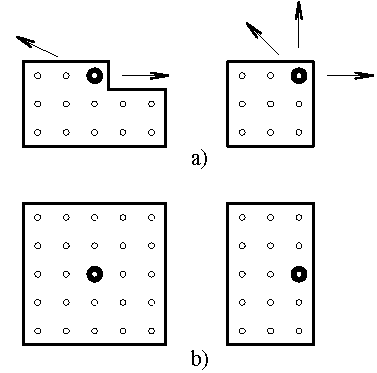
\includegraphics[scale=1.0]{05_filtrace/images/img_5_2.pdf}
    \end{center}
    \caption{a) Funkce $c(m, n)$ umožňující přímý výpočet, b) neumožňující přímý výpočet.}
    \label{img:5_2}
\end{figure}

Pro „nastartování`` výpočtu rekurzivního filtru je třeba mít předem k dispozici některé hodnoty výstupního obrazu \textit{g}. Tyto hodnoty mají význam okrajových podmínek. Požadujeme-li filtr lineární, pak je nutné jako okrajové podmínky zadávat pouze hodnoty 0. Toto tvrzení vyplývá z jednoduché úvahy: Nechť $\mathscr{O}$ je uvažovaný rekurzivní filtr. Předpokládejme, že filtr $\mathscr{O}$ je lineární. Platí proto

\begin{equation} \label{eq:5_28}
    \mathscr{O} \left\{ af(m, n) \right\} = a \mathscr{O} \left\{ f(m, n) \right\}.
\end{equation}

Položíme-li v \eqref{eq:5_28} \textit{a}=0, konstatujeme na základě uvedeného vztahu, že v~případě lineárního filtru nulovému vstupnímu obrazu nutně odpovídá také nulový obraz výstupní. Při volbě nenulových okrajových podmínek by zde obecně došlo ke sporu: nulovému vstupnímu obrazu by odpovídal nenulový obraz výstupní, a proto by filtr $\mathscr{O}$ nebyl lineární. Ani poloha bodů, ve kterých zadáváme okrajové podmínky, nemůže být volena libovolně. Okrajové podmínky, lze zadávat pouze v těch místech, kde hodnotu výstupního pole neurčuje výraz \eqref{eq:5_24}. Obr. \ref{img:5_3} ukazuje příklady míst, v nichž se zadávají okrajové podmínky, pro různé tvary oblasti, nad níž je funkce \textit{c} nenulová.

\begin{figure}[th]
    \begin{center}
        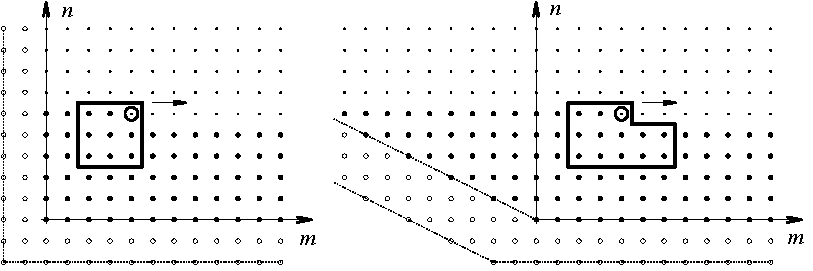
\includegraphics[scale=0.88]{05_filtrace/images/img_5_3.pdf}
    \end{center}
    \caption{Příklady okrajových podmínek pro různé funkce $c(m, n)$.}
    \label{img:5_3}
\end{figure}

Na rozdíl od nerekurzivních filtrů, které jsou vždy stabilní, je u filtrů rekurzivních nutno sledovat problémy stability. Jestliže je filtr nestabilní, pak se v~průběhu výpočtu mohou šířit zaokrouhlovací chyby a případné šumy vstupního pole a dosahovat vysokých hodnot. Tento problém byl v~minulosti detailně studován, ale jeho podrobnější diskuse by přesáhla rámec tohoto textu. V~případě zájmu proto čtenáře odkazujeme např. na práci (Dudgeon 84).

\subsection*{Realizace rekurzivního filtru iteračním výpočtem}

\noindent V předchozím odstavci jsme vysvětlili, že má-li oblast, nad níž funkce \textit{b,c} nabývají nenulové hodnoty, vhodný tvar, pak lze rekurzivní filtraci realizovat přímým výpočtem. Ne všechny filtry jsou ovšem takto realizovatelné. Přímý výpočet nelze uplatnit tehdy, jestliže by pro výpočet hodnoty \textit{g}(\textit{m},\textit{n}) bylo zapotřebí hodnot v těch místech výstupního pole, kde zatím nebyly vypočteny. V těchto případech lze však použít iteračního postupu. Na základě vztahu \eqref{eq:5_24} se pro výpočet \textit{g}(\textit{m},\textit{n}) nabízí iterační předpis

\begin{equation} \label{eq:5_29}
    g_i(m, n) = a(m, n) * f(m, n) + c(m, n) * g_{i-1} (m, n),
\end{equation}
kde \textit{gi}(\textit{m},\textit{n}) znamená hodnotu v~\textit{i}-tém iteračním kroku. Pro zahájení iteračního pochodu volíme \textit{g}$_0$(\textit{m},\textit{n}) = 0. Oprávněnost iteračního postupu popsaného vztahem \eqref{eq:5_29} je ovšem samozřejmě nutné doložit studiem konvergence. Ačkoli předpokládáme, že samotný výpočet filtrace bude prováděn v~prostorové doméně, analýzu konvergence provedeme v~doméně frekvenční. Fourierovou transformací vztahu \eqref{eq:5_24} obdržíme

\begin{equation} \label{eq:5_30}
    G(k, l) = A(k, l) F(k, l) + C(k, l) G(k, l),
\end{equation}
kde \textit{C} je Fourierovou transformací funkce \textit{c}. Z \eqref{eq:5_30} dostaneme dále vztah

\begin{equation} \label{eq:5_31}
    G(k, l) = \frac{A(k, l)}{1 - C(k, l)} F(k, l).
\end{equation}

Fourierovou transformací rovnice \eqref{eq:5_29} získáme

\begin{equation} \label{eq:5_32}
    G_i(k, l) = A(k, l) F(k, l) + C(k, l) G_{i-1}(k, l).
\end{equation}

Odtud máme

\begin{eqnarray} \label{eq:5_33}
    G_1(k, l) &=& A(k, l) F(k, l), \quad G_2(k, l) = A(k, l) F(k, l) \left[ 1 + C(k, l) \right],\\
    G_n(k, l) &=& A(k, l) F(k, l) \sum\limits_{i=0}^{n-1} C^i(k, l). \nonumber
\end{eqnarray}

S využitím identity,

\begin{equation} \label{eq:5_34}
    \sum\limits_{i=0}^{n-1} C^i(k, l) = \frac{1 - C^n(k, l)}{1 - C(k, l)},
\end{equation}
za předpokladu že \textbar \textit{C}(\textit{k},\textit{l})\textbar  $<$ 1 a s~uplatněním vztahu \eqref{eq:5_31} docházíme v případě nekonečného počtu iteračních kroků k~následujícímu závěru:

\begin{equation} \label{eq:5_35}
    \lim\limits_{n \rightarrow \infty} G_n(k, l) = A(k, l) F(k, l) \lim\limits_{n \rightarrow \infty} \frac{1 - C^n(k, l)}{1 - C(k, l)} = \frac{A(k, l)}{1 - C(k, l)} F(k, l) = G(k, l).
\end{equation}

Vidíme tedy, že jestliže platí \textbar \textit{C}(\textit{k},\textit{l})\textbar  $<$ 1, pak iterační proces konverguje k přesnému řešení. Poznamenejme však, že uvedená podmínka je zbytečně přísná. Podrobnější analýzou bylo totiž dokázáno, že iteračním postupem lze realizovat každý stabilní filtr (Dudgeon 84).

\subsection*{Návrh rekurzivního filtru}

Návrhem rekurzivního filtru rozumíme stanovení funkcí \textit{a}(\textit{m},\textit{n}), \textit{b}(\textit{m},\textit{n}) tak, aby měl filtr požadované vlastnosti. Výchozími údaji pro návrh může být např. nějaký vstupní signál \textit{f}(\textit{m},\textit{n}) a požadovaná odezva \textit{d}(\textit{m},\textit{n}) filtru na tento signál (příkladem je realizace filtru se~zadanou impulzovou charakteristikou). Naznačme postup takového návrhu. Aby časová složitost filtrace byla co nejmenší, požadujeme, aby funkce \textit{a},\textit{b} měly nenulové funkční hodnoty jen v~malém počtu bodů. Nechť \textit{g}(\textit{m},\textit{n}) je skutečná odezva filtru na funkci \textit{f}(\textit{m},\textit{n}). S~ohledem na předchozí požadavek se bude skutečná odezva lišit od odezvy požadované. Úhrnná kvadratická chyba filtru v prostorové doméně pak je

\begin{equation} \label{eq:5_36}
    \epsilon \sum\limits_{m} \sum\limits_{n} \left[ g(m, n) - d(m, n) \right]^2.
\end{equation}

Funkce \textit{a}(\textit{m},\textit{n}), \textit{b}(\textit{m},\textit{n}) stanovíme minimalizací funkcionálu \eqref{eq:5_36}. Analogický postup můžeme realizovat také ve frekvenční doméně. Úhrnná kvadratická chyba filtru ve frekvenční doméně je

\begin{equation} \label{eq:5_37}
    \epsilon = \sum\limits_{k} \sum\limits_{l} \left[ G(k, l) - D(k, l) \right]^2 = \sum\limits_{k} \sum\limits_{l} \left[ \frac{A(k, l)}{B(k, l)} F(k, l) - D(k, l) \right]^2.
\end{equation}

Můžeme také zavést funkci $W_{k, l}$ vyjadřující váhu chyby pro jednotlivé frekvence. Máme pak

\begin{equation} \label{eq:5_38}
    \epsilon_\mathrm{W} = \sum\limits_{k} \sum\limits_{l} W_{k, l} \left[ \frac{A(k, l)}{B(k, l)} F(k, l) - D(k, l) \right]^2.
\end{equation}

Poznamenejme na závěr, že ať již použijeme návrhu v doméně prostorové nebo frekvenční, jsou rezultující úlohy minimalizace nelineární, a proto je zde zpravidla zapotřebí použít numerického řešení.

\section*{Obecný model degradace a rekonstrukce obrazu}

Při snímání obrazu často dochází k jeho různým poškozením (degradacím). Obraz může být např. zašumělý, neostrý atd. Pokud je to možné, bývá obvykle žádoucí tyto degradace korigovat. Korekce bývá dosti často realizována filtrací. Klíčovou otázkou je volba vhodného filtru. K jeho nalezení je nejprve vhodné zavést model degradace obrazu. Označme \textit{f}$_\mathrm{I}$ vstupní nepoškozený obraz. Obraz \textit{f}$_\mathrm{I}$ není ovšem k dispozici. Dostupný je místo něj pouze obraz poškozený, který označíme \textit{f}$_\mathrm{D}$. Představujeme si, že degradace je způsobena nějakým operátorem (označme jej $\mathscr{D}$) a dále si představujeme, že dochází k degradaci aditivním šumem (označme jej \textit{v}). Je tedy

\begin{equation} \label{eq:5_39}
    f_\mathrm{D} = \mathscr{D} \left\{ f_\mathrm{I} \right\} + v.
\end{equation}

Úkolem rekonstrukce obrazu je nalézt rekonstrukční operátor $\mathscr{R}$ tak, abychom jeho aplikací na obraz \textit{f}$_\mathrm{D}$ obdrželi obraz (označme jej \textit{f}$_\mathrm{R}$), který je co možná nejbližší obrazu \textit{f}$_\mathrm{I}$. Máme tedy

\begin{equation} \label{eq:5_40}
    f_\mathrm{R} = \mathscr{R} \left\{ f_\mathrm{D} \right\} = \mathscr{R} \left\{ \mathscr{D} \left\{ f_\mathrm{I} \right\} + v \right\}.
\end{equation}

Ze všech možných operátorů zvolíme za operátor $\mathscr{R}$ ten, který dává minimální hodnotu chyby

\begin{equation} \label{eq:5_41}
    \epsilon = || f_\mathrm{R} - f_\mathrm{I} ||.
\end{equation}

Předpokládejme nyní, že degradační operátor $\mathscr{D}$ je lineární a invariantní vůči posuvu. Jeho impulzovou a frekvenční charakteristiku označme \textit{h}$_\mathrm{D}$, \textit{H}$_\mathrm{D}$. Také rekonstrukční operátor $\mathscr{R}$ předpokládáme lineární a invariantní vůči posuvu. Úkolem je nalézt impulzovou charakteristiku \textit{h}$_\mathrm{R}$ nebo frekvenční charakteristiku \textit{H}$_\mathrm{R}$ rekonstrukčního operátoru $\mathscr{R}$ tak, aby byla minimalizována chyba ze vztahu \eqref{eq:5_41}. Zapišme rovnice \eqref{eq:5_39}, \eqref{eq:5_40} pomocí konvoluce. Máme

\begin{equation} \label{eq:5_42}
    f_\mathrm{D} (m, n) = f_\mathrm{I} (m, n) * h_\mathrm{D} (m, n) + v(m, n),
\end{equation}

\begin{equation} \label{eq:5_43}
    f_\mathrm{R} (m, n) = \left[ f_\mathrm{I} (m, n) * h_\mathrm{D} (m, n) + v(m, n) \right] * h_\mathrm{R}(m, n).
\end{equation}

Provedeme-li Fourierovu transformaci uvedených vztahů, dostaneme

\begin{equation} \label{eq:5_44}
    F_\mathrm{D} (k, l) = F_\mathrm{I} (k, l) H_\mathrm{D} (k, l) + V(k, l).
\end{equation}

\begin{equation} \label{eq:5_45}
    F_\mathrm{R} (k, l) = \left[ F_\mathrm{I} (k, l) H_\mathrm{D} (k, l) + V(k, l) \right] H_\mathrm{R}(k, l).
\end{equation}

\section*{Inverzní filtrace}

O inverzním filtru hovoříme tehdy, jestliže frekvenční charakteristiku rekonstrukčního operátoru $\mathscr{R}$ zvolíme ve tvaru

\begin{equation} \label{eq:5_46}
    H_\mathrm{R} (k, l) = \frac{1}{H_\mathrm{D} (k, l)}.
\end{equation}

Dosazením vztahu \eqref{eq:5_46} do \eqref{eq:5_45} zjišťujeme, že platí

\begin{equation} \label{eq:5_47}
    F_\mathrm{R} (k, l) = F_\mathrm{I} (k, l) + \frac{V(k, l)}{H_\mathrm{D}(k, l)}.
\end{equation}

Inverzní Fourierovou transformací pak obdržíme

\begin{equation} \label{eq:5_48}
    f_\mathrm{R} (m, n) = f_\mathrm{I} (m, n) + \mathscr{F}^{-1} \left\{ \frac{V(k, l)}{H_\mathrm{D}(k, l)} \right\}.
\end{equation}

Ze vztahu \eqref{eq:5_48} vidíme, že pokud by obraz \textit{f}$_\mathrm{D}$ nebyl degradován šumem, pak by inverzní filtr poskytl obraz, který je shodný s nepoškozeným vstupním obrazem \textit{f}$_\mathrm{I}$. Za přítomnosti šumu se ovšem obrazy \textit{f}$_\mathrm{R}$ a \textit{f}$_\mathrm{I}$ liší. Odchylka je popsána druhým členem na pravé straně rovnice \eqref{eq:5_48}. Je zřejmé, že vliv šumu roste s tím, jak klesají hodnoty \textit{H}$_\mathrm{D}$(\textit{k}, \textit{l}). Protože u většiny degradací jsou hodnoty \textit{H}$_\mathrm{D}$(\textit{k},\textit{l}) odpovídající vyšším frekvenčním složkám, kde vliv šumu zejména očekáváme, malé (obraz je obvykle rozostřován tím, že jsou potlačeny vyšší frekvence), dochází použitím inverzního filtru často k nežádoucímu zdůraznění šumu. Jiným praktickým problémem je, že frekvenční charakteristiku degradačního operátoru mnohdy neznáme přesně. Často je nutné spokojit se s pouhým odhadem.

\section*{Wienerův filtr ve frekvenční doméně}

V~této podkapitole využijeme k~nalezení rekonstrukčního filtru stochastického přístupu. Ukážeme nejprve odvození tzv. Wienerova filtru ve frekvenční doméně (v prostorové doméně jej odvodíme v~následující podkapitole). Předpokládáme, že \textbf{f}$_\mathrm{I}$(\textit{m},\textit{n}), \textbf{f}$_\mathrm{D}$(\textit{m},\textit{n}), \textbf{f}$_\mathrm{R}$(\textit{m},\textit{n}) jsou homogenní náhodná pole rozměru \textit{M}$\times$\textit{N} reprezentující postupně ideální, degradovaný a rekonstruovaný obraz a že \textbf{v}(\textit{m},\textit{n}) je náhodné pole rozměru \textit{M}$\times$\textit{N}, které reprezentuje aditivní šum. Také odpovídající Fourierovy obrazy \textbf{F}$_\mathrm{I}$(\textit{m},\textit{n}), \textbf{F}$_\mathrm{D}$(\textit{m},\textit{n}), \textbf{F}$_\mathrm{R}$(\textit{m},\textit{n}), \textbf{V}(\textit{m},\textit{n}) jsou náhodná pole rozměru \textit{M}$\times$\textit{N}. Pro zestručnění položme

\begin{equation} \label{eq:5_49}
    \mathbf{f}_\Delta (m, n) = f_\mathrm{R} (m, n) - \mathbf{f}_\mathrm{I} (m, n),
\end{equation}

\begin{equation} \label{eq:5_50}
    \mathbf{F}_\Delta (k, l) = \mathscr{F} \left\{ \mathbf{f}_\Delta (m, n) \right\} = \mathbf{F}_\mathrm{r} (k, l) - \mathbf{F}_\mathrm{I}(k, l).
\end{equation}

Rekonstrukční filtr nalezneme minimalizací chyby

\begin{equation} \label{eq:5_51}
    \epsilon = \mathrm{E} \left\{ \sum\limits_{m=0}^{M-1} \sum\limits_{n=0}^{N-1} | \mathbf{f}_\Delta (m, n) |^2 \right\}.
\end{equation}

Podle Parsevalova teorému \eqref{eq:2_59} ovšem platí

\begin{equation} \label{eq:5_52}
    \epsilon = \mathrm{E} \left\{ \sum\limits_{m=0}^{M-1} \sum\limits_{n=0}^{N-1} | \mathbf{f}_\Delta (m, n) |^2 \right\} = \mathrm{E} \left\{ \sum\limits_{m=0}^{M-1} \sum\limits_{n=0}^{N-1} | \mathbf{F}_\Delta (k, l) |^2 \right\}.
\end{equation}

\textbf{F}$_\Delta$(\textit{k},\textit{l}) vyjádříme dosazením vztahu \eqref{eq:5_45} do vztahu \eqref{eq:5_50}. Dostaneme

\begin{equation} \label{eq:5_53}
    \mathbf{F}_\Delta (k, l) = \left[ \mathbf{F}_\mathrm{I} (k, l) H_\mathrm{D} (k, l) + \mathbf{V}(k, l) \right] H_\mathrm{D}(k, l) - \mathbf{F}_\mathrm{I}(k, l).
\end{equation}

Uvážíme-li, že $|\mathbf{F}_\Delta(k, l)|^2 = \mathbf{F}_\Delta(k, l)\mathbf{F}_\Delta^*(k, l)$, pak ze vztahu \eqref{eq:5_52} máme

\begin{equation} \label{eq:5_54}
    \epsilon = \mathrm{E} \left\{ \sum\limits_{k=0}^{M-1} \sum\limits_{l=0}^{N-1} | \mathbf{F}_\Delta (k, l) \mathbf{F}_\Delta^* (k, l) \right\}.
\end{equation}

Frekvenční charakteristiku \textit{H}$_\mathrm{R}$ rekonstrukčního filtru určíme z podmínky

\begin{equation} \label{eq:5_55}
    \frac{\partial\epsilon}{\partial H_\mathrm{R}(r, s)} = 0, \,\,\, r = 0, 1, \dots, M-1, \,\,\, s = 0, 1, \dots, N-1.
\end{equation}

Ze vztahu \eqref{eq:5_54} máme

\begin{eqnarray} \label{eq:5_56}
    \frac{\partial\epsilon}{\partial H_\mathrm{R}(r, s)} &=& \mathrm{E} \left\{ \sum\limits_{k=0}^{M-1} \sum\limits_{l=0}^{N-1} \left[ \frac{\partial\mathbf{F}_\Delta (k, l)}{\partial H_\mathrm{R}(r, s)} \mathbf{F}_\Delta^* (k, l) + \mathbf{F}_\Delta (k, l) \frac{\partial F_\Delta^*(k, l)}{\partial H_\mathrm{R}(r, s)} \right] \right\} \\
    &=& \mathrm{E} \left\{ \frac{\partial\mathbf{F}_\Delta (r, s)}{\partial H_\mathrm{R}(r, s)} \mathbf{F}_\Delta^* (r, s) + \mathbf{F}_\Delta (r, s) \frac{\partial F_\Delta^*(r, s)}{\partial H_\mathrm{R}(r, s)}\right\}. \nonumber
\end{eqnarray}

Předpokládejme, že náhodná pole \textbf{f}$_\mathrm{I}$, \textbf{v} jsou nekorelovaná. Uplatněním výsledku z podkapitoly \ref{sec:statisticka_analyza_obrazovych_transformaci} lze snadno ukázat, že pole \textbf{F}$_\mathrm{I}$(\textit{k}, \textit{l}) a \textbf{V}(\textit{k},\textit{l}) jsou proto také nekorelovaná, z čehož vyplývá E\{\textbf{F}$_\mathrm{I}$(\textit{k},\textit{l})\textbf{V}(\textit{k},\textit{l})\} = E\{\textbf{F}$_\mathrm{I}$(\textit{k},\textit{l})\}E\{\textbf{V}(\textit{k},\textit{l})\}. Dále předpokládejme, že E\{\textbf{v}(\textit{m},\textit{n})\} = 0. Odtud plyne, že E\{\textbf{V}(\textit{k},\textit{l})\} = 0. Dosadíme-li do vztahu \eqref{eq:5_56} vztah \eqref{eq:5_53}, položíme-li E\{\textbf{F}$_\mathrm{I}$(\textit{k},\textit{l})\textbf{F}$_\mathrm{I}^*$(\textit{k},\textit{l})\}/$\surd$(\textit{MN}) = \textit{G}$_{\mathrm{f}_\mathrm{I} \mathrm{f}_\mathrm{I}}$(\textit{k},\textit{l}), E\{\textbf{V}(\textit{k},\textit{l}) \textbf{V}$^*$(\textit{k},\textit{l})\}/$\surd$(\textit{MN}) = \textit{G}$_{\mathrm{vv}}$(\textit{k},\textit{l}), pak po úpravách dostaneme pro rekonstrukční filtr předpis

\begin{equation} \label{eq:5_57}
    H_\mathrm{R}(r, s) = H_\mathrm{D}^*(r, s) \frac{G_{\mathrm{f}_\mathrm{I} \mathrm{f}_\mathrm{I}}(r, s)}{|H_\mathrm{D}(r, s)|^2 G_{\mathrm{f}_\mathrm{I} \mathrm{f}_\mathrm{I}}(r, s) + G_{\mathrm{vv}}(r, s)}.
\end{equation}

Poznamenejme, že $G_{\mathrm{f}_\mathrm{I} \mathrm{f}_\mathrm{I}}$ je výkonová spektrální hustota vstupního nedegradovaného signálu a $G_{\mathrm{vv}}$ je výkonová spektrální hustota šumu (viz. výsledek příkladu 3.1).

%\section*{Wienerův filtr v prostorové doméně}

%\noindent V~této podkapitole ukážeme odvození Wienerova filtru v~prostorové doméně. Opět předpokládáme, že \textbf{f}I, \textbf{f}D, \textbf{f}R jsou homogenní náhodná pole reprezentující ideální, degradovaný a rekonstruovaný obraz a že \textbf{v} je náhodné pole popisující aditivní šum. Stejně jako v~předchozí podkapitole, je i zde cílem nalézt filtr, který na základě znalosti degradovaného obrazu provede jeho rekonstrukci, která je v jistém smyslu optimální. Abychom mohli použít přehledného maticového zápisu, reprezentujme všechna uvedená pole pomocí sloupcových vektorů rozměru \textit{MN}. Předpokládáme, že odhad bude možné vyjádřit ve tvaru

% , \eqref{GrindEQ__5_58_}

%\noindent kde \textbf{W} je zatím neznámá matice rozměru \textit{MN}$\times$\textit{MN} a \textbf{b} je zatím neznámý vektor rozměru \textit{MN}, které musíme stanovit tak, aby byl odhad optimální. Požadujeme, aby střední hodnota odhadu byla stejná jako střední hodnota ideálního obrazu, tedy aby platilo

% . \eqref{GrindEQ__5_59_}

%\noindent Dále požadujme, aby odhad \textbf{f}R minimalizoval chybu

% . \eqref{GrindEQ__5_60_}

%\noindent Ekvivalentním postupem k~minimalizaci chyby ze vztahu \eqref{GrindEQ__5_60_} je aplikace principu ortogonality. Podle tohoto principu můžeme hledanou matici \textbf{W} a vektor \textbf{b} nalézt pomocí následující podmínky

% . \eqref{GrindEQ__5_61_}

%\noindent Protože jsme princip ortogonality uvedli bez důkazu, pokusme se alespoň o jeho poněkud méně formální, avšak názornou interpretaci: Jestliže jsou chyba odhadu (rozdíl v první kulaté závorce) a odchylka pozorování od střední hodnoty (rozdíl v druhé kulaté závorce) nekorelované veličiny, pak již použitými prostředky (statistické momenty druhého řádu) nelze nic zlepšovat. Pro stručnost a  přehlednost zápisu zaveďme označení

% ,   . \eqref{GrindEQ__5_62_}

%\noindent Ze vztahu \eqref{GrindEQ__5_58_} a z podmínky \eqref{GrindEQ__5_59_} snadno získáme předpis

% . \eqref{GrindEQ__5_63_}

%\noindent Dosadíme-li do podmínky ortogonality \eqref{GrindEQ__5_61_} vztah \eqref{GrindEQ__5_58_} a \eqref{GrindEQ__5_63_}, pak postupně dostaneme

%  \eqref{GrindEQ__5_64_}

% ,

%\noindent kde \textbf{C}fDfD, \textbf{C}fIfD jsou kovarianční matice. Ze vztahu \eqref{GrindEQ__5_64_} pak dále máme

% . \eqref{GrindEQ__5_65_}

%\noindent Předpokládejme nyní, že vstupní obraz \textbf{f}I je degradován lineárním operátorem reprezentovaným maticí \textbf{D} a šumem reprezentovaným vektorem \textbf{v}. Pro degradovaný obraz \textbf{f}D proto můžeme psát

% . \eqref{GrindEQ__5_66_}

%\noindent Uplatníme-li na vztah \eqref{GrindEQ__5_66_} operaci střední hodnoty a výsledek dosadíme do vztahu \eqref{GrindEQ__5_63_}, máme

% , \eqref{GrindEQ__5_67_}

%\noindent kde v je vektor středních hodnot šumu. Dosazením vztahu \eqref{GrindEQ__5_66_} do \eqref{GrindEQ__5_65_} dále máme

% . 

%  \eqref{GrindEQ__5_68_}

%\noindent Jestliže jsou náhodná pole \textbf{f}I a \textbf{v} navzájem nekorelovaná, vychází

% . \eqref{GrindEQ__5_69_}

%\noindent Uvedený vztah můžeme dále zjednodušit za předpokladu, že pro každé dva různé body obrazu je ideální signál i šum nekorelovaný. V tomto případě jsou kovarianční matice \textbf{C}fIfI, \textbf{C}vv diagonální. Zaveďme další zjednodušení a předpokládejme kovarianční matice ve tvaru

% ,   , \eqref{GrindEQ__5_70_}

%\noindent kde \textbf{I} je jednotková matice. Ze vztahu \eqref{GrindEQ__5_69_} pak dostaneme předpis

% . \eqref{GrindEQ__5_71_}

